\chapter{Ensayos y mediciones}

\section{Medición de ripple.}

Para poder realizar las siguiente mediciones en este primer ensayo, previamente se realizo en la placa la soldadura del puente diodo y el filtro.

\subsection{En el filtro capacitivo y determinación de parámetros.}

Se tomaran medidas de la tension tanto desde el punto bajo (desde 0 hasta 10 V) como desde el punto alto (desde 15 hasta 30 V) variando la corriente desde el vacio (0 A) hasta llegar a plena carga (1,5 A). Con las mediciones vamos a poder calcular los siguientes tres factores: Regulacion de voltaje, resistencia variable y factor de ripple.\\

Punto bajo:

\begin{table}[H]
  \centering
  \begin{tabular}{|c|c|}
    \hline
    $V_{vacio}$ & 17,71 V \\ \hline
    $V_{0,5 A}$ & 15,80 V \\ \hline
    $V_{0,75 A}$ & 15,27 V \\ \hline    
    $V_{1 A}$ & 14,63 V \\ \hline
    $V_{1,25 A}$ & 14,10 V \\ \hline
    $V_{PlenaCarga}$ & 13,69 V \\ \hline
  \end{tabular}
\end{table}


\begin{figure}[H]
  \centering
  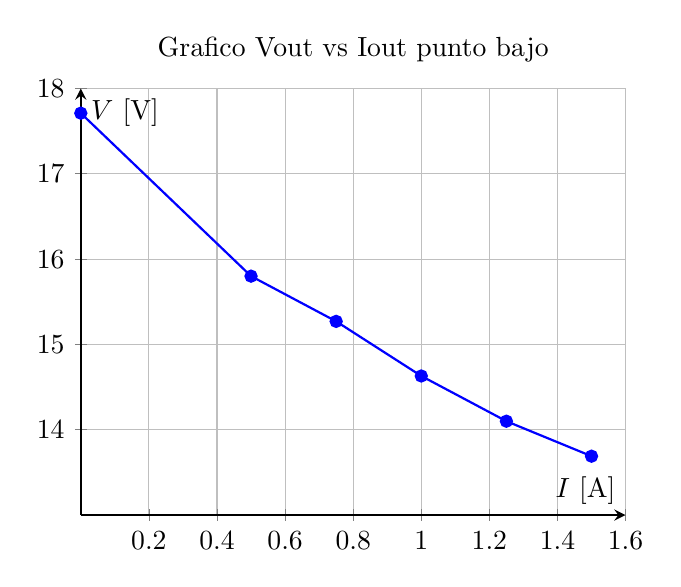
\begin{tikzpicture}
    \begin{axis}[
      axis lines = middle,
      xlabel = {$I$ [A]},
      ylabel = {$V$ [V]},
      domain = 0:1.5,
      samples = 200,
      grid = both,
      width=8.5cm,
      height=7cm,
      title = {Grafico Vout vs Iout punto bajo},
      xmin = 0, xmax= 1.6,
      ymin = 13, ymax = 18,
      thick
      ]
      \addplot[blue, mark=*] coordinates {
            (0, 17.71)
            (0.5, 15.80)
            (0.75, 15.27)
            (1, 14.63)
            (1.25, 14.10)
            (1.5, 13.69)
      };
    \end{axis}
  \end{tikzpicture}
\end{figure}


Punto alto:

\begin{table}[H]
  \centering
  \begin{tabular}{|c|c|}
    \hline
    $V_{vacio}$ & 36,86 V \\ \hline
    $V_{0,5 A}$ & 31,89 V \\ \hline
    $V_{0,75 A}$ & 31,05 V \\ \hline    
    $V_{1 A}$ & 29,83 V \\ \hline
    $V_{1,25 A}$ & 28,55 V \\ \hline
    $V_{PlenaCarga}$ & 27,47 V \\ \hline
  \end{tabular}
\end{table}

\begin{figure}[H]
  \centering
  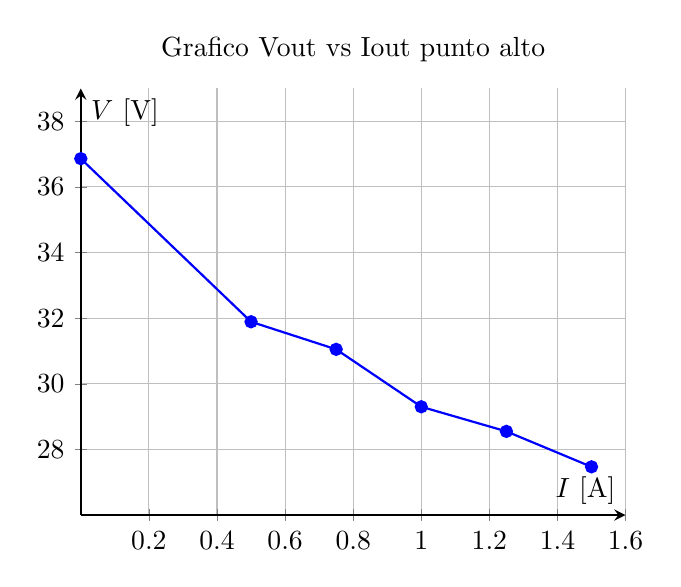
\begin{tikzpicture}
    \begin{axis}[
      axis lines = middle,
      xlabel = {$I$ [A]},
      ylabel = {$V$ [V]},
      domain = 0:1.5,
      samples = 200,
      grid = both,
      width=8.5cm,
      height=7cm,
      title = {Grafico Vout vs Iout punto alto},
      xmin = 0, xmax= 1.6,
      ymin = 26, ymax = 39,
      thick
      ]
      \addplot[blue, mark=*] coordinates {
            (0, 36.86)
            (0.5, 31.89)
            (0.75, 31.05)
            (1, 29.3)
            (1.25, 28.55)
            (1.5, 27.47)
      };
    \end{axis}
  \end{tikzpicture}
\end{figure}

\subsection{Determinación de resistencia interna del transformador más la de los diodos.}

Punto bajo: \\

\begin{itemize}

  \item Para calcular la regulacion de voltaje se utiliza la siguiente formula: \\

$RV = \dfrac{V_{vacio} - V_{PlenaCarga}}{V_{PlenaCarga}} 100\percent $

$RV = \dfrac{17,71 - 13,69}{13,69} 100\percent = 29,36\percent $\\

  \item La resistencia interna esta dada por: \\

$R_int = \dfrac{V_{PlenaCarga} - V_{vacio}}{-I_{carga}}$

$R_int = \dfrac{13,69 - 17,71}{-1,5} = 2,68\Omega $\\

  \item Ahora mediremos el voltaje del ripple tanto con multimetro true RMS, como en el osciloscopio: \\

$V_{RippleMultimetro} = 908 mV$

$V_{RippleOsciloscopio} = 972 mV$

$V_{PicoaPico} = 2,75 V$ \\

  \item Factor de ripple: \\

$F_R = \dfrac{V_{eficaz}}{V_{PlenaCarga}} 100\percent $

$F_R = \dfrac{908 mV}{13,69 V} 100\percent $

$F_R = 6,6325\percent $ \\

Para el punto alto repetiremos las formulas del punto bajo cambiando por los valores correspondientes: \\

  \item Regulacion de voltaje: \\

$RV = \dfrac{36,68 - 27,43}{27,43} 100\percent = 33,72\percent $\\

  \item Resistencia interna:

$R_int = \dfrac{27,43 - 36,68}{-1,5} = 6,16\Omega $\\

  \item Ripple:

$V_{RippleMultimetro} = 0,83 V$

$V_{RippleOsciloscopio} = 0,88 V$

$V_{PicoaPico} = 2,5 V$ \\

  \item Factor de ripple:

$F_R = \dfrac{0,83 V}{27,43 V} 100\percent $

$F_R = 3,0258 $ \\

\end{itemize}

\section{Mediciones finales.}

Antes de continuar con las ultimas mediciones, se debera soldar el resto de la placa, osea; el regulador lm317, la fuente auxiliar, las borneras que conectan al potenciometro y el led. A continuacion mediremos la caida de tension en el lm317 y la corriente para llevarlo a su maxima potencia la cual es 15 W, luego mediremos la tension en el vacio y a plena carga para calcular la regulacion de voltaje, a continuacion observaremos la salida a plena carga por el osciloscopio para calcular la tension eficaz del ripple y calcular el factor de ripple, y por ultimo mediremos la temperatura en la carcasa del regulador para poder determinar su temperatura interna.  \\

\begin{figure}[h]
  \centering
  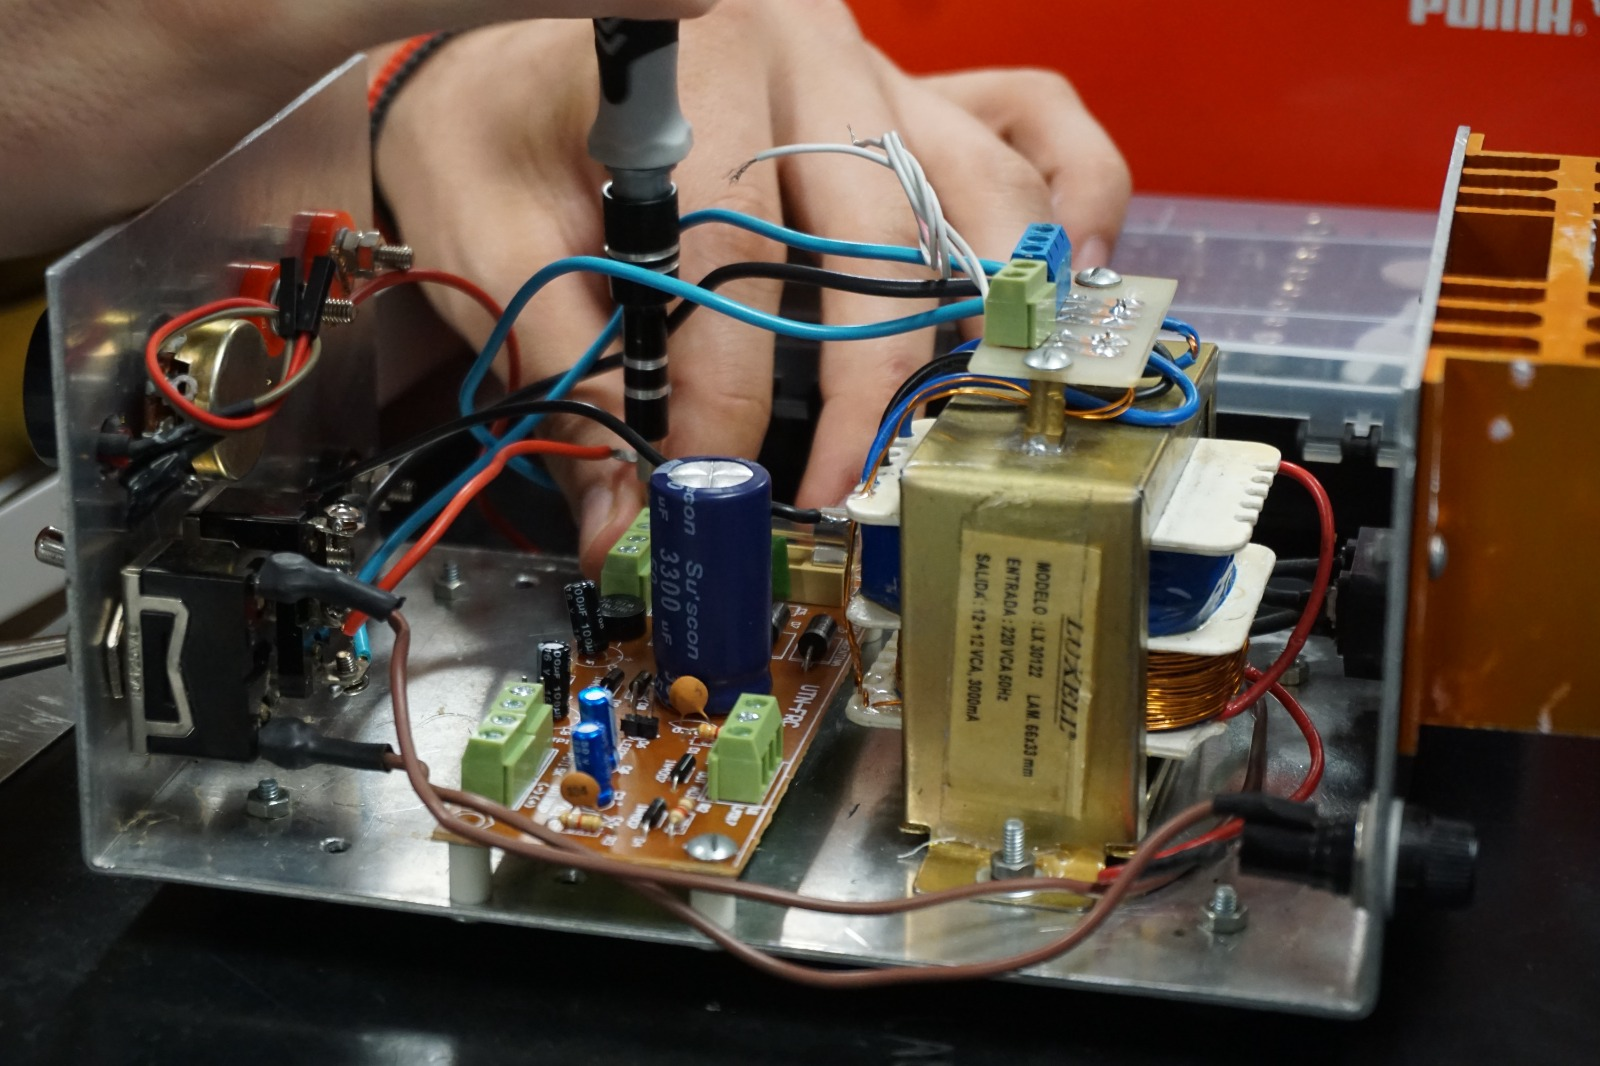
\includegraphics[width=0.70\textwidth]{images/placaMontada.png}
\end{figure}

\subsection{Regulación de voltaje.}

\begin{table}[H]
  \centering
  \begin{tabular}{|c|c|}
    \hline
    $V_{vacio}$ & 16,92 V \\ \hline
    $V_{PlenaCarga}$ & 16,29 V \\ \hline
  \end{tabular}
\end{table}

$RV = \dfrac{16,92 - 16,29}{16,29} 100\percent$

$RV = 3,867 $

\subsection{Factor de ripple.}

$V_{RippleEficaz} = 353,55 . 10^{-6} V = 353,5 uV $

$F_R = \dfrac{353,5 uV}{16,29 V} 100\percent $

$F_R = 2,1703 . 10^{-3}\percent $ \\

\begin{figure}[H]
  \centering
  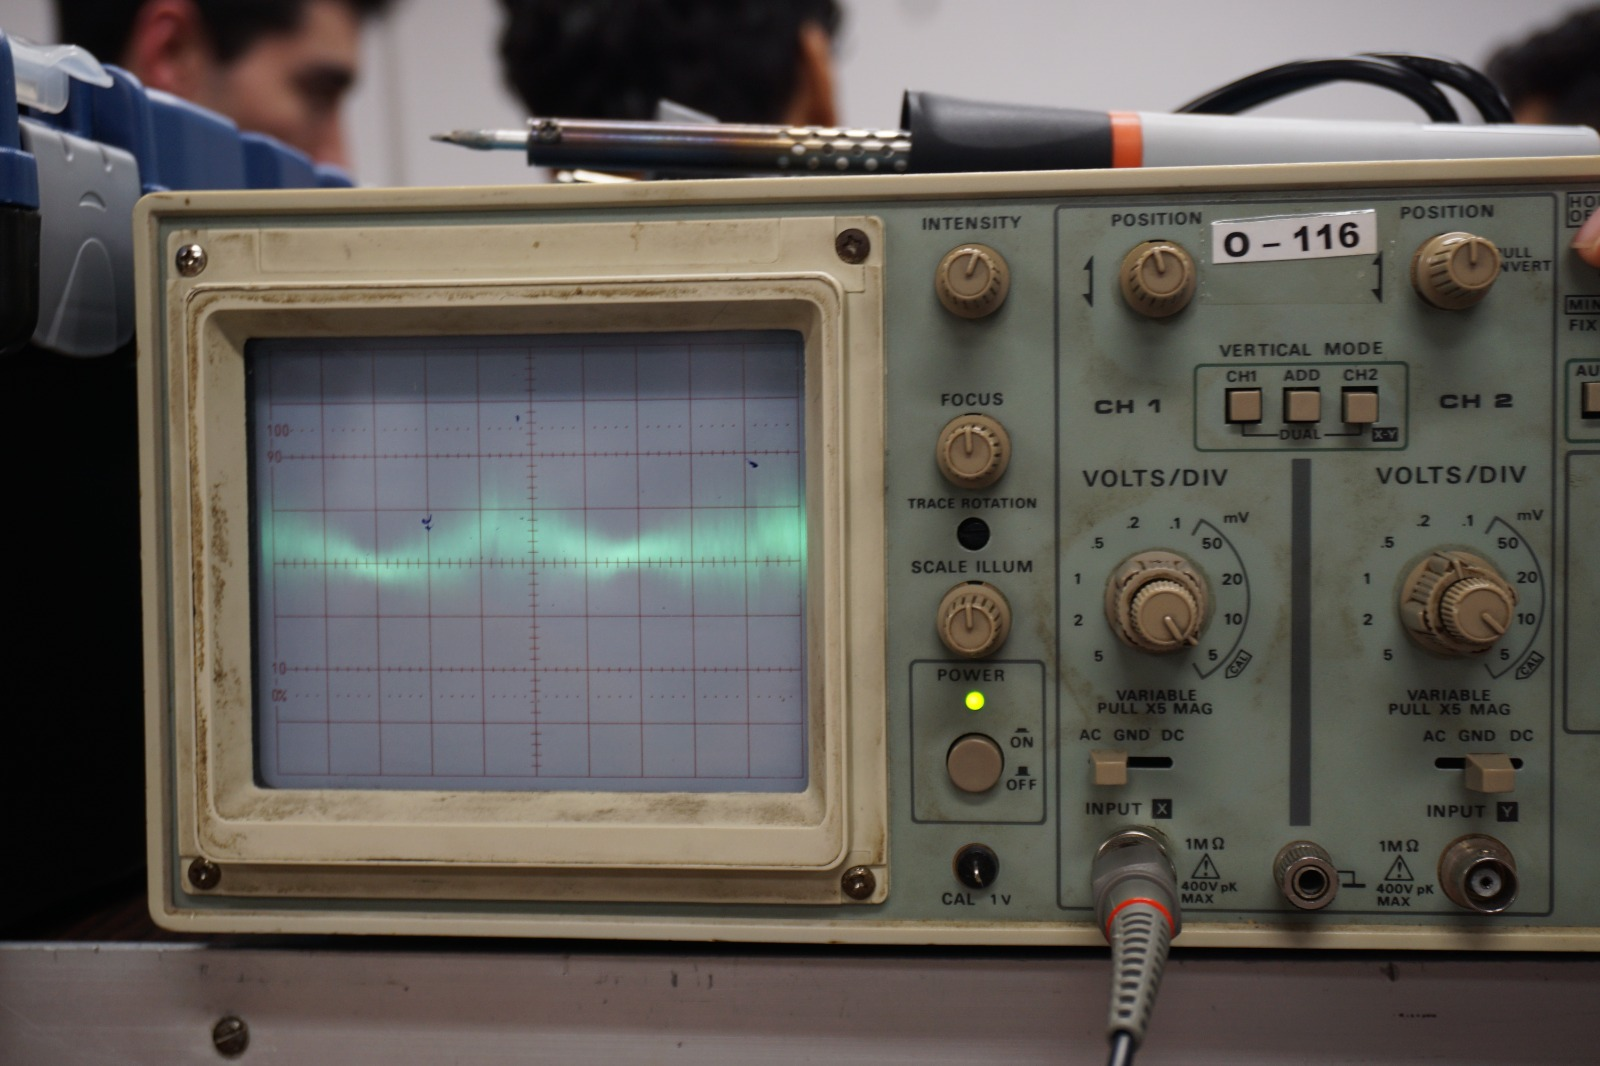
\includegraphics[width=0.70\textwidth]{images/medicionRipple.png}
  \caption{Visualizacion de riple en osciloscopio}
\end{figure}


\subsection{Cálculo de temperatura de juntura.}

\begin{figure}[H]
  \centering
  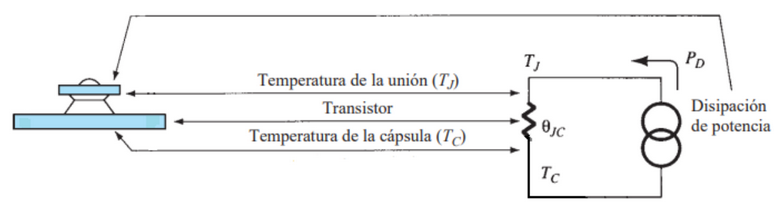
\includegraphics[width=0.95\textwidth]{images/calculoTemperatura.png}
  \caption{Calculo de la temperatura}
\end{figure}

Siendo: \\

$\theta_{jc} = 5\dfrac{\circ C}{W} $ : Resistencia termica de la juntura \\

$T_J = 135 \circ C$ : Temperatura de la juntura \\

$135 \circ C = (5 \dfrac{\circ C}{W} 15,19 W) + T_C $

$135 \circ C - 75 \circ C = T_C$

$T_C = 60 \circ C$ : Temperatura del chip

\begin{figure}[H]
  \centering
  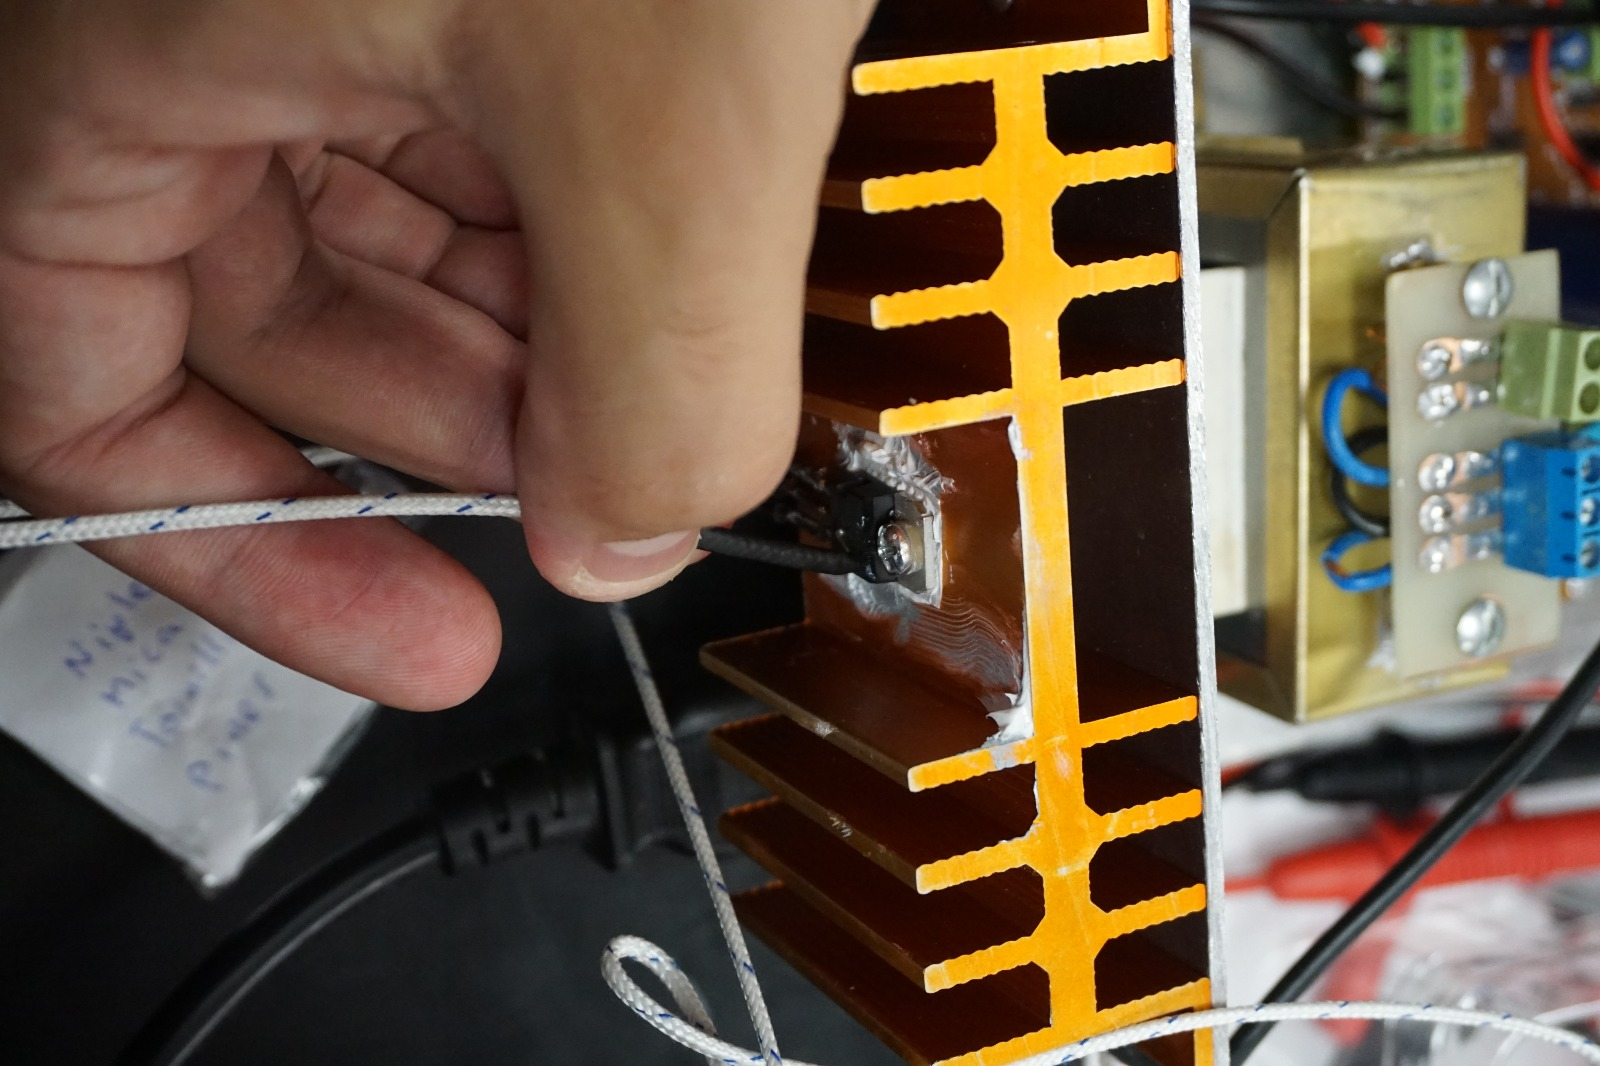
\includegraphics[width=0.70\textwidth]{images/medicionTemperatura.png}
  \caption{Medicion de la tempera en LM317}
\end{figure}

